\documentclass[tikz,border=5pt]{standalone}
\usepackage{tikz}
\usetikzlibrary{positioning}

\begin{document}
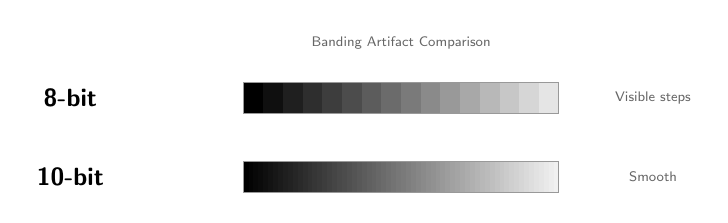
\begin{tikzpicture}[
    label/.style={font=\small\sffamily\bfseries},
    sublabel/.style={font=\tiny\sffamily, text=black!60}
]

% 8-bit gradient with banding
\begin{scope}[shift={(0,0)}]
    \node[label] at (-2.2, 0) {8-bit};

    % Stepped gradient (banding visible)
    \foreach \i in {0,...,15} {
        \pgfmathsetmacro{\gray}{100 - \i*6}
        \fill[black!\gray] (\i*0.25, -0.2) rectangle (\i*0.25+0.25, 0.2);
    }
    \draw[black!40] (0, -0.2) rectangle (4, 0.2);

    \node[sublabel] at (5.2, 0) {Visible steps};
\end{scope}

% 10-bit gradient (smoother)
\begin{scope}[shift={(0,-1)}]
    \node[label] at (-2.2, 0) {10-bit};

    % Smooth gradient
    \foreach \i in {0,...,63} {
        \pgfmathsetmacro{\gray}{100 - \i*1.5}
        \fill[black!\gray] (\i*0.0625, -0.2) rectangle (\i*0.0625+0.0625, 0.2);
    }
    \draw[black!40] (0, -0.2) rectangle (4, 0.2);

    \node[sublabel] at (5.2, 0) {Smooth};
\end{scope}

% Title
\node[sublabel] at (2, 0.7) {Banding Artifact Comparison};

\end{tikzpicture}
\end{document}
